\documentclass[border=0.2cm, 12pt]{standalone}
\usepackage{tikz}
\usepackage{amsmath, amssymb, amsfonts, mathtools}
\usepackage{color}

\usetikzlibrary{shapes,snakes}
\tikzset{>=latex}

\begin{document}
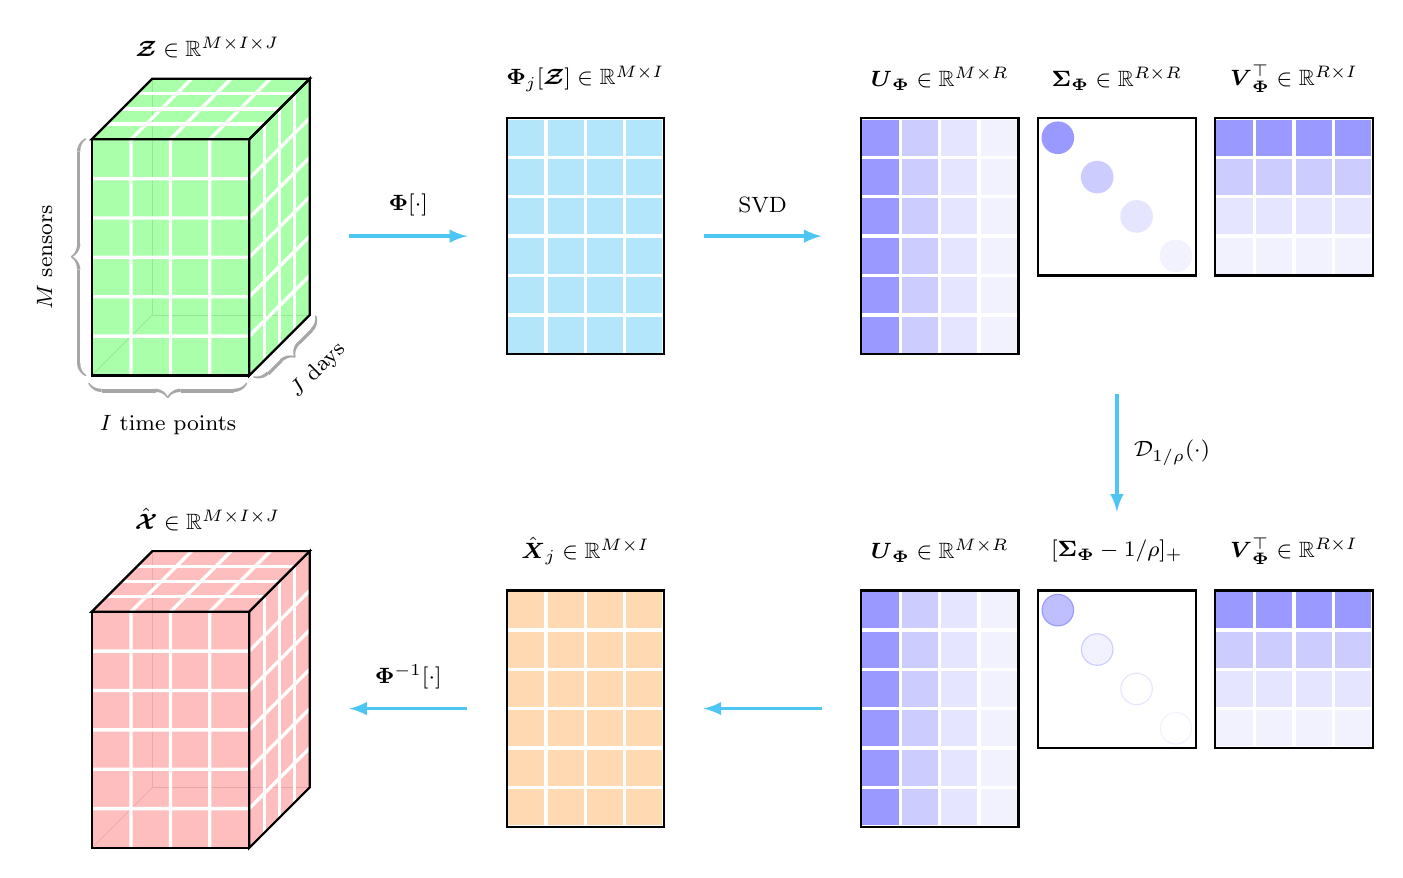
\begin{tikzpicture}
  
\newcommand{\Depth}{2}
\newcommand{\Height}{2}
\newcommand{\Width}{3}

\coordinate (O) at (0,0,0);
\coordinate (A) at (0,\Width,0);
\coordinate (B) at (0,\Width,\Height);
\coordinate (C) at (0,0,\Height);
\coordinate (D) at (\Depth,0,0);
\coordinate (E) at (\Depth,\Width,0);
\coordinate (F) at (\Depth,\Width,\Height);
\coordinate (G) at (\Depth,0,\Height);
\draw[gray,very thin,fill=green!5] (O) -- (C) -- (G) -- (D) -- cycle;% Bottom Face
\draw[gray,very thin,fill=green!5] (O) -- (A) -- (E) -- (D) -- cycle;% Back Face
\draw[gray,very thin,fill=green!5] (O) -- (A) -- (B) -- (C) -- cycle;% Left Face
\draw[fill=green!40,opacity=0.8] (D) -- (E) -- (F) -- (G) -- cycle;% Right Face
\draw[fill=green!40,opacity=0.8] (C) -- (B) -- (F) -- (G) -- cycle;% Front Face
\draw[fill=green!40,opacity=0.8] (A) -- (B) -- (F) -- (E) -- cycle;% Top Face

\draw[white, very thick] (0,0.5,2) -- (2,0.5,2) -- (2,0.5,0);
\draw[white, very thick] (0,1,2) -- (2,1,2) -- (2,1,0);
\draw[white, very thick] (0,1.5,2) -- (2,1.5,2) -- (2,1.5,0);
\draw[white, very thick] (0,2,2) -- (2,2,2) -- (2,2,0);
\draw[white, very thick] (0,2.5,2) -- (2,2.5,2) -- (2,2.5,0);

\draw[white, very thick] (0.5,0,2) -- (0.5,3,2) -- (0.5,3,0);
\draw[white, very thick] (1,0,2) -- (1,3,2) -- (1,3,0);
\draw[white, very thick] (1.5,0,2) -- (1.5,3,2) -- (1.5,3,0);

\draw[white, very thick] (2,0,1.5) -- (2,3,1.5) -- (0,3,1.5);
\draw[white, very thick] (2,0,1) -- (2,3,1) -- (0,3,1);
\draw[white, very thick] (2,0,0.5) -- (2,3,0.5) -- (0,3,0.5);


\draw[black,thick] (D) -- (E) -- (F) -- (G) -- cycle;% Right Face
\draw[black,thick] (C) -- (B) -- (F) -- (G) -- cycle;% Front Face
\draw[black,thick] (A) -- (B) -- (F) -- (E) -- cycle;% Top Face

\draw (0.2,-1.2-0.2,0) node {\footnotesize{\color{black}\text{$I$~time points}}};
\draw (0.2,-0.95,0) node[rotate = 0] {{\color{black!35}$\underbrace{\hspace{2cm}}$}};
\draw (-0.6,1.5,2) node[rotate = 90] {\footnotesize{\color{black}\text{$M$~sensors}}};
\draw (-0.15,1.5,2) node[rotate = 270] {{\color{black!35}$\underbrace{\hspace{3cm}}$}};
\draw (2.6,-0.2,1.3) node[rotate = 45] {\footnotesize{\color{black}\text{$J$~days}}};
\draw (2.2,0,1.2) node[rotate = 45] {{\color{black!35}$\underbrace{\hspace{1.1cm}}$}};

\node at (0.7,3.4) {\footnotesize\color{black}$\boldsymbol{\mathcal{Z}}\in\mathbb{R}^{M\times I\times J}$};

\draw[very thick,color=cyan!70,latex-] (4,1) -- (2.5,1); % ultra
\node at (3.25,1.4) {\footnotesize\color{black}$\boldsymbol{\Phi}[\cdot]$};

\newcommand{\temp}{4.5}

\filldraw [fill=cyan!30!white,draw=green!40!black] (\temp,0-0.5) rectangle (\temp+2,3-0.5);
\draw [step=0.5, very thick, color=white] (\temp+0,0-0.5) grid (\temp+2,3-0.5);
\draw [thick] (\temp,0-0.5) rectangle (\temp+2,3-0.5);

\node at (\temp+1,3.0) {\footnotesize\color{black}$\boldsymbol{\Phi}_{j}[\boldsymbol{\mathcal{Z}}]\in\mathbb{R}^{M\times I}$};

\draw[very thick,color=cyan!70,latex-] (\temp+4,1) -- (\temp+2.5,1); % ultra
\node at (\temp+3.25,1.4) {\footnotesize\color{black}SVD};

%%% Left singular vectors
\newcommand{\leftsv}{\temp+4.5}

\filldraw [fill=blue!40!white,draw=green!40!black] (\leftsv,0-0.5) rectangle (\leftsv+0.5,3-0.5);
\filldraw [fill=blue!20!white,draw=green!40!black] (\leftsv+0.5,0-0.5) rectangle (\leftsv+1,3-0.5);
\filldraw [fill=blue!10!white,draw=green!40!black] (\leftsv+1,0-0.5) rectangle (\leftsv+1.5,3-0.5);
\filldraw [fill=blue!5!white,draw=green!40!black] (\leftsv+1.5,0-0.5) rectangle (\leftsv+2,3-0.5);
\draw [step=0.5, very thick, color=white] (\leftsv+0,0-0.5) grid (\leftsv+2,3-0.5);
\draw [thick] (\leftsv,0-0.5) rectangle (\leftsv+2,3-0.5);

\node at (\leftsv+1,3.0) {\footnotesize\color{black}$\boldsymbol{U}_{\boldsymbol{\Phi}}\in\mathbb{R}^{M\times R}$};

%%% Singular values
\newcommand{\sv}{\temp+6.75}

\node[circle,draw=blue!40,fill=blue!40,inner sep=0pt,minimum size=0.4cm] (sv1) at (\sv+0.25,3-0.5-0.25) {};
\node[circle,draw=blue!20,fill=blue!20,inner sep=0pt,minimum size=0.4cm] (sv1) at (\sv+0.25+0.5,3-0.5-0.25-0.5) {};
\node[circle,draw=blue!10,fill=blue!10,inner sep=0pt,minimum size=0.4cm] (sv1) at (\sv+0.25+1,3-0.5-0.25-1) {};
\node[circle,draw=blue!5,fill=blue!5,inner sep=0pt,minimum size=0.4cm] (sv1) at (\sv+0.25+1.5,3-0.5-0.25-1.5) {};
\draw [thick] (\sv,1-0.5) rectangle (\sv+2,3-0.5);

\node at (\sv+1,3.0) {\footnotesize\color{black}$\boldsymbol{\Sigma}_{\boldsymbol{\Phi}}\in\mathbb{R}^{R\times R}$};

%%% Right singular vectors
\newcommand{\rightsv}{\temp+9}

\filldraw [fill=blue!40!white,draw=green!40!black] (\rightsv,2.5-0.5) rectangle (\rightsv+2,3-0.5);
\filldraw [fill=blue!20!white,draw=green!40!black] (\rightsv,2-0.5) rectangle (\rightsv+2,2.5-0.5);
\filldraw [fill=blue!10!white,draw=green!40!black] (\rightsv,1.5-0.5) rectangle (\rightsv+2,2-0.5);
\filldraw [fill=blue!5!white,draw=green!40!black] (\rightsv,1-0.5) rectangle (\rightsv+2,1.5-0.5);
\draw [step=0.5, very thick, color=white] (\rightsv+0,1-0.5) grid (\rightsv+2,3-0.5);
\draw [thick] (\rightsv,1-0.5) rectangle (\rightsv+2,3-0.5);

\node at (\rightsv+1,3.0) {\footnotesize\color{black}$\boldsymbol{V}_{\boldsymbol{\Phi}}^\top\in\mathbb{R}^{R\times I}$};

\draw[very thick,color=cyan!70,latex-] (\temp+6.75+1,-2.5) -- (\temp+6.75+1,-1); % ultra
\node at (\temp+6.75+1.7,-1.75) {\footnotesize\color{black}$\mathcal{D}_{1/\rho}(\cdot)$};

\newcommand{\down}{-6}
%%% Left singular vectors

\filldraw [fill=blue!40!white,draw=green!40!black] (\leftsv,0-0.5+\down) rectangle (\leftsv+0.5,3-0.5++\down);
\filldraw [fill=blue!20!white,draw=green!40!black] (\leftsv+0.5,0-0.5+\down) rectangle (\leftsv+1,3-0.5+\down);
\filldraw [fill=blue!10!white,draw=green!40!black] (\leftsv+1,0-0.5+\down) rectangle (\leftsv+1.5,3-0.5+\down);
\filldraw [fill=blue!5!white,draw=green!40!black] (\leftsv+1.5,0-0.5+\down) rectangle (\leftsv+2,3-0.5+\down);
\draw [step=0.5, very thick, color=white] (\leftsv+0,0-0.5+\down) grid (\leftsv+2,3-0.5+\down);
\draw [thick] (\leftsv,0-0.5+\down) rectangle (\leftsv+2,3-0.5+\down);

\node at (\leftsv+1,3.0+\down) {\footnotesize\color{black}$\boldsymbol{U}_{\boldsymbol{\Phi}}\in\mathbb{R}^{M\times R}$};

%%% Singular values

\node[circle,draw=blue!40,fill=blue!25,inner sep=0pt,minimum size=0.4cm] (sv1) at (\sv+0.25,3-0.5-0.25+\down) {};
\node[circle,draw=blue!20,fill=blue!5,inner sep=0pt,minimum size=0.4cm] (sv1) at (\sv+0.25+0.5,3-0.5-0.25-0.5+\down) {};
\node[circle,draw=blue!10,fill=blue!0,inner sep=0pt,minimum size=0.4cm] (sv1) at (\sv+0.25+1,3-0.5-0.25-1+\down) {};
\node[circle,draw=blue!5,fill=blue!0,inner sep=0pt,minimum size=0.4cm] (sv1) at (\sv+0.25+1.5,3-0.5-0.25-1.5+\down) {};
\draw [thick] (\sv,1-0.5+\down) rectangle (\sv+2,3-0.5+\down);

\node at (\sv+1,3.0+\down) {\footnotesize\color{black}$[\boldsymbol{\Sigma}_{\boldsymbol{\Phi}}-1/\rho]_{+}$};

%%% Right singular vectors

\filldraw [fill=blue!40!white,draw=green!40!black] (\rightsv,2.5-0.5+\down) rectangle (\rightsv+2,3-0.5+\down);
\filldraw [fill=blue!20!white,draw=green!40!black] (\rightsv,2-0.5+\down) rectangle (\rightsv+2,2.5-0.5+\down);
\filldraw [fill=blue!10!white,draw=green!40!black] (\rightsv,1.5-0.5+\down) rectangle (\rightsv+2,2-0.5+\down);
\filldraw [fill=blue!5!white,draw=green!40!black] (\rightsv,1-0.5+\down) rectangle (\rightsv+2,1.5-0.5+\down);
\draw [step=0.5, very thick, color=white] (\rightsv+0,1-0.5+\down) grid (\rightsv+2,3-0.5+\down);
\draw [thick] (\rightsv,1-0.5+\down) rectangle (\rightsv+2,3-0.5+\down);

\node at (\rightsv+1,3.0+\down) {\footnotesize\color{black}$\boldsymbol{V}_{\boldsymbol{\Phi}}^\top\in\mathbb{R}^{R\times I}$};

\draw[very thick,color=cyan!70,-latex] (\temp+4,1+\down) -- (\temp+2.5,1+\down); % ultra

\draw[very thick,color=cyan!70,-latex] (4,1+\down) -- (2.5,1+\down); % ultra
\node at (3.25,1.4+\down) {\footnotesize\color{black}$\boldsymbol{\Phi}^{-1}[\cdot]$};

\filldraw [fill=orange!30!white,draw=green!40!black] (\temp,0-0.5+\down) rectangle (\temp+2,3-0.5+\down);
\draw [step=0.5, very thick, color=white] (\temp+0,0-0.5+\down) grid (\temp+2,3-0.5+\down);
\draw [thick] (\temp,0-0.5+\down) rectangle (\temp+2,3-0.5+\down);

\node at (\temp+1,3.0+\down) {\footnotesize\color{black}$\hat{\boldsymbol{X}}_{j}\in\mathbb{R}^{M\times I}$};

\coordinate (O) at (0,0+\down,0);
\coordinate (A) at (0,\Width+\down,0);
\coordinate (B) at (0,\Width+\down,\Height);
\coordinate (C) at (0,0+\down,\Height);
\coordinate (D) at (\Depth,0+\down,0);
\coordinate (E) at (\Depth,\Width+\down,0);
\coordinate (F) at (\Depth,\Width+\down,\Height);
\coordinate (G) at (\Depth,0+\down,\Height);
\draw[gray,very thin,fill=red!5] (O) -- (C) -- (G) -- (D) -- cycle;% Bottom Face
\draw[gray,very thin,fill=red!5] (O) -- (A) -- (E) -- (D) -- cycle;% Back Face
\draw[gray,very thin,fill=red!5] (O) -- (A) -- (B) -- (C) -- cycle;% Left Face
\draw[fill=red!30,opacity=0.8] (D) -- (E) -- (F) -- (G) -- cycle;% Right Face
\draw[fill=red!30,opacity=0.8] (C) -- (B) -- (F) -- (G) -- cycle;% Front Face
\draw[fill=red!30,opacity=0.8] (A) -- (B) -- (F) -- (E) -- cycle;% Top Face

\draw[white, very thick] (0,0.5+\down,2) -- (2,0.5+\down,2) -- (2,0.5+\down,0);
\draw[white, very thick] (0,1+\down,2) -- (2,1+\down,2) -- (2,1+\down,0);
\draw[white, very thick] (0,1.5+\down,2) -- (2,1.5+\down,2) -- (2,1.5+\down,0);
\draw[white, very thick] (0,2+\down,2) -- (2,2+\down,2) -- (2,2+\down,0);
\draw[white, very thick] (0,2.5+\down,2) -- (2,2.5+\down,2) -- (2,2.5+\down,0);

\draw[white, very thick] (0.5,0+\down,2) -- (0.5,3+\down,2) -- (0.5,3+\down,0);
\draw[white, very thick] (1,0+\down,2) -- (1,3+\down,2) -- (1,3+\down,0);
\draw[white, very thick] (1.5,0+\down,2) -- (1.5,3+\down,2) -- (1.5,3+\down,0);

\draw[white, very thick] (2,0+\down,1.5) -- (2,3+\down,1.5) -- (0,3+\down,1.5);
\draw[white, very thick] (2,0+\down,1) -- (2,3+\down,1) -- (0,3+\down,1);
\draw[white, very thick] (2,0+\down,0.5) -- (2,3+\down,0.5) -- (0,3+\down,0.5);


\draw[black,thick] (D) -- (E) -- (F) -- (G) -- cycle;% Right Face
\draw[black,thick] (C) -- (B) -- (F) -- (G) -- cycle;% Front Face
\draw[black,thick] (A) -- (B) -- (F) -- (E) -- cycle;% Top Face

\node at (0.7,3.4+\down) {\footnotesize\color{black}$\hat{\boldsymbol{\mathcal{X}}}\in\mathbb{R}^{M\times I\times J}$};


\end{tikzpicture}
\end{document}